\documentclass[a4paper,11 pt,fleqn]{report}
\usepackage[utf8]{inputenc}
\usepackage{lmodern}
\usepackage[frenchb]{babel}
\usepackage[top=2.5cm,bottom=2.5cm,right=2.5cm,left=2.5cm]{geometry}
\usepackage{array}
\usepackage{color}
\usepackage{url}

\usepackage{graphicx}
\usepackage{sectsty}
\usepackage{titlesec}

\title{\textbf{Projet Génie Logiciel} \vspace{3\baselineskip}\\
  Rapport du Projet\vspace{2\baselineskip}}
\author{Bastien Lepesant, Arya Jemo et Lucas Nicosia.}
\date{25 Mai 2015}

\graphicspath{{Images/}}

\begin{document}

  \def\chaptername{Partie}

  \sectionfont{\large}

  \titleformat{\chapter}[display]{\normalfont\huge\bfseries}{}{20pt}{\huge}

  \titlespacing*{\chapter}{0pt}{-50pt}{10pt}
 
  \maketitle
  \tableofcontents
 
  \chapter{Introduction}
    \section{Contexte}
  Dans le cadre de notre deuxième année de licence en Informatique, nous avons l'opportunité de participer au projet Génie Logiciel encadré par M. Tianxiao LIU.
  Celui-ci consiste en la réalisation et la conception d'un logiciel java beaucoup plus complexe et de plus grande ambition que ceux réalisés jusqu'à maintenant.
  Nous avons eu a chance d'obtenir notre premier choix lors de la sélection des projets, soit le sujet \textbf{Conquête}.
  
  \subsection{Objet}
  Notre objectif est de réaliser un jeu de stratégie multijoueurs. Dans celui-ci, chaque joueur se voit attribuer une capitale puis tour à tour, 
  chacun des joueurs va conquérir des territoires neutres ou ennemis à l'aide de soldats. Le gagnant est celui qui à conquérit toutes les capitales.
 Toutefois notre projet implique des mécanismes plus complexes afin de répondre au cahier des charges, tels que des alliances entre joueurs, le jeu en réseau ainsi que d'autres fonctionnalités que nous allons décrire dans ce rapport.
  \subsection{Équipe}
  Notre équipe est composé de trois CMI SIC\footnote{Cursus Master en Ingénierie, systèmes intelligents et communicants} :
  \begin{itemize}
    \item Arya Jemo
    \item Bastien Lepesant
    \item Lucas Nicosia
  \end{itemize}
  
  \chapter{Spécification}
    \section{Cahier des Charges}
	
  \subsection{Calendrier}

  Durant toute la durée du projet, nous avons un calendrier précis à respecter :  \\ \\
  %Création du tableau	
  \begin{tabular}{|c|c|c|}
  \hline \textbf{Semaine du : } & \textbf{Objectif} \\
  \hline 19 Janvier & Cahier des charges \\
  \hline 26 Janvier & UML modèle \\
  \hline 02 Février & UML moteur \\
  \hline 09 Février &Prototype graphique \\
  \hline 02 Mars & \textbf{Point d'avancement 1 : démo du prototype du projet} \\
  \hline 09 Mars & Mise en place Junit + Log4j \\
  \hline 23 Mars & Mise en place rédaction LaTex \\
  \hline 06 Avril & Squelette des slides \\
  \hline 13 Avril & \textbf{Point d'avancement 2 : pré-soutenance du projet} \\
  \hline 18 Mai & Finalisation du projet + \textbf{Remise de projet ( au plus tard le 24 mai )} \\
  \hline 25 Mai & \textbf{Soutenances de projet : Mardi 26 et Mercredi 27 Mai} \\
  \hline 
  \end{tabular}
  %Fin Tableau
	
  \subsection{Environnement de travail}
  Durant le projet, nous allons utiliser les outils suivants ( sur nos ordinateurs personnels ) : \begin{itemize}
  \item L'IDE Java \textbf{Eclipse}
  \item Le logiciel de gestion de versions \textbf{SVN}.
  \end{itemize}

\section{Objectif du projet}

  \subsubsection{Solution envisagée}
    Dans toute cette partie, nous ajouterons de la couleur suivante \textcolor{red}{\textbf{les objectifs bonus que nous aimerions réaliser si le temps nous le permet}}.
    Comme résultat final, nous voulons obtenir un jeu jouable sur Linux, Windows et Mac. Ce dernier doit comporter un moteur de jeu, un moteur graphique et permettre de jouer contre d'autres joueurs et/ou contre l'ordinateur.
    \textcolor{red}{\textbf{Le jeu est jouable en réseau, à plusieurs.}}
  \subsubsection{Méthodes envisagées}

  L'idée du jeu que nous voulons réaliser peut se diviser en 3 parties : 
  \begin{itemize}
    \vspace{1cm}
    \item \textbf{\underline{Menu de jeu}} : Lors du lancement du jeu, le logiciel affichera en premier temps un Menu permettant au joueur de réaliser les actions suivantes : 
    
      \begin{itemize}
  
	\item Lancer une nouvelle partie.
	\item Charger une partie existante ( ou supprimer une sauvegarde existante ).
	\item Quitter le jeu.
  
      \end{itemize}
    \vspace{1cm}
    \item \textbf{\underline{Génération de carte}} : Notre logiciel devra permettre la génération d'une carte de jeu, composée d'un ensemble de territoires ayant chacun 2 caractéristiques  liées: 
      \begin{itemize}
	\item Une réserve des trois ressources différentes du jeu : nourriture, or et bois.
	\item Une production différente pour chacune des trois ressources
      \end{itemize}
      De plus, chaque joueur disposera {d'une capitale}, l'unique premier territoire  lui appartenant ( la capitale dispose des mêmes caractéristiques que les autres territoires ). 
      La génération évitera que deux capitales soient directement voisines au début du jeu. Le reste des territoires sera neutre.
      Lors du lancement d'une partie, le joueur aura la possibilité de générer la map avec 3 modes différents : 
      \begin{itemize}
	\item \textbf{Mode normal} : Il peut choisirs 3 paramètres, et le logiciel se charge du reste :
	
	\begin{itemize}
	  \item Le nombre de joueurs.
	  \item Le taux de production durant tout le jeu  : faible, moyenne, importante, etc.
	  \item L'emplacement des capitales : Soit il les pose lui même, soit elles le sont aléatoirement.
	\end{itemize}
  
	\item \textbf{Mode aléatoire} : Tous les paramètres du jeu sont fixés de manière totalement aléatoire, sans aucune contrainte : le nombre de joueurs, l'ordre des tours de chaque joueur, l'emplacement des capitales, la réserve et la production de chaque territoire, etc.
	\item \textbf{Mode éditeur} : Ouverture d'un mode édition, permettant la modification des tous les paramètres de la partie : nombre de joueurs ( un nombre maximum sera tout de même fixé ), emplacement des capitales, réserve et production de chaque territoire, etc.
      \end{itemize}
    \vspace{1cm}
    \item \textbf{\underline{Moteur de jeu}} : Lorsqu'une partie démarre, chaque joueur a donc une capitale. Le jeu se déroule au tour par tour, sur la même machine. Suivant le choix de création de la carte, un ordre de jeu entre les joueurs est défini. Durant le tour d'un joueur, celui-ci peut réaliser différentes actions, réparties en 2 phases :
      \begin{itemize}
	\vspace{0.5cm}
	\item \textbf{Phase de Gestion} : Le joueur peut : 
	  \begin{itemize} 
	    \item \underline{Créer un bâtiment} ( unique ) sur chacun de ses territoires. Il existe 3 types de bâtiments, chacun ayant des caractéristiques et un temps de construction différents : 
	      \begin{itemize}
		\item Le Bâtiment de production : celui-ci augmente la production de toutes les ressources du territoire en question de X \% ( X reste à définir pour des questions d'équilibrage ).
		\item La Caserne : ce bâtiment sert à la production de soldats.
		\textcolor{red}{\textbf{Plusieurs types de bâtiments militaires, associés à différents groupes de soldats: Caserne, Ecurie, etc.}}
		\item Le Bastion : ce bâtiment octroie un bonus de défense aux troupes présentes sur le territoire en question.
	      \end{itemize}
	    \underline{N.B} : Les capitales sont considérées comme possédant chacun des 3 bâtiments. Elles ont donc une production accélérée et une défense augmentée par 
	      rapport aux autres territoires. Elles permettent aussi la production de soldats.
	    \item \underline{Produire des soldats} : Sur chaque territoire possédant une caserne, le joueur peut lancer la production d'un bataillon de soldats. 
	      Chaque soldat dispose d'une valeur d'attaque et d'une valeur de défense. Il existe plusieurs types d'unités différents ( ex : guerrier, chevalier, roi, etc ). 
	      Par conséquent, chaque unité dispose d'un temps de construction propre, d'un nombre de soldats par bataillon propre, et d'une valeur d'attaque et de défense propres. 
	      Toutes ces informations ne sont pas encore fixées pour des raisons d'équilibrage.
	    \item \underline{Déplacer ses soldats} : Chaque bataillon peut se déplacer d'un territoire par tour. Les déplacements sur les territoires alliés ( les territoires alliés comprennent 
	      ceux du joueur ET ceux de ses alliés ) sont sans conséquences. Les déplacements sur un territoire ennemi ou neutre vide entraînent la capture immédiate de celui-ci. Les déplacements 
	      sur un territoire occupé par des unités ennemies entraîneront un combat lors de la phase en question. Le vainqueur capturera le territoire.
	    \item \underline{Gérer ses alliances} : Le joueur peut demander à n'importe quel autre la création d'un pacte. Dès lors, le jeu demande au potentiel allié sa réponse, directement 
	      pendant le tour du premier ( ceci permet de n'avantager personne lors de la phase de gestion ). A l'inverse, il peut choisir de rompre un pacte déjà existant. Dans ce cas, 
	      l'autre joueur concerné n'est pas informé jusqu'à la phase de combat et devra anticiper ou deviner en fonction des déplacements du traitre.
	      Toutes les informations de relations entre les différents pays et leurs frontières seront traitées à l'aide de graphes.
	  \end{itemize}
	\vspace{0.5cm}
	\item \textbf{Phase de Combat} :
	  La deuxième phase consiste à la réalisation des combats. Celle-ci se déroule en même temps pour tous les joueurs. Pour commencer, les ruptures d'alliance sont annoncées. Le programme analyse la carte, et pour chaque territoire où au moins deux unités non alliées sont présentes simultanément, un combat a lieu. Ceci comprend le cas où deux unités alliées se trouvent sur le même territoire, mais l'un des deux joueurs a rompu le pacte pendant sa phase de gestion.
	  Le déroulement d'un combat est divisé en plusieurs étapes :
      
	  \begin{itemize}
	    \item Calcul des valeurs de combat des joueurs : pour chaque joueur différent présent dans le combat, une valeur de combat est calculée. Celle-ci est obtenue en multipliant le nombre de soldats de chaque type par la valeur d'attaque de ce type. Dans le cas où le territoire où se déroule le combat appartient à un joueur, ce sont les valeurs de défense de ses soldats qui sont prises en compte.
	      \textcolor{red}{\textbf{Intégration d'unités maritimes, combats navales et amélioration du gameplay.}}
	    \item Une fois les valeurs de combat calculées, le jeu affiche le pourcentage de chances de chaque joueur de remporter le combat.
	      Dans le cas où deux joueurs sont alliés, on additionne leurs valeurs.
	    \item Enfin, l'issue du combat est calculée à partir des chances de chacun des joueurs de gagner. Les unités de tous les perdants sont détruites, le gagnant capture le territoire. Dans le cas où les attaquants sont des alliés, celui qui avait la plus grande valeur de combat obtient le territoire, l'autre obtient X  \% ( X reste à définir pour des questions d'équilibrage ) des productions en ressources du territoire.
	  \end{itemize}
	  Une fois tous les combats effectués, le tour suivant peut commencer avec la phase de gestion du premier joueur.
	  
      \end{itemize}
      Pendant une partie, le joueur doit avoir accès à un menu lui permettant de sauvegarder sa partie, d'en charger une autre ou enfin de quitter.
    \vspace{1cm}
    \item \textbf{\underline{Moteur Graphique}} : Notre logiciel sera capable de gérer un moteur graphique. Celui-ci aura pour but d'afficher à l'écran toutes les informations nécéssaires à l'utilisateur pour jouer. Cela comprend les options suivantes :
      \begin{itemize}
	\item Affichage des menus, avec boutons.
	\item Affichage de la carte vue de dessus, des différents territoires avec surlignage des frontières, ainsi que des troupes ( de même pour le mode édition ).
	  Chaque joueur sera représenté d'une couleur différente.
	\item Permettre à l'utilisateur de séléctionner ses territoires et ses troupes afin d'y effectuer les actions de son choix. Affichage d'un menu diplomatique 
	  afin d'y ajouter ou de rompre des alliances.
	\item Lors de la phase de combat, affichage des informations et des résultats de chaque combat.

      \end{itemize}

    \vspace{1cm}
    \item \textbf{\underline{Ambiance sonore}} : 
      \textcolor{red}{\textbf{Ajout de musiques d'ambiances différentes selon les niveaux.}}

    \vspace{1cm}
    \item \textbf{\underline{IA}} : Le jeu devra permettre, lors de la séléction du nombre de joueurs, de choisir de jouer contre l'ordinateur. Il proposera alors plusieurs niveaux de difficultés correspondants à des IAs de plus en plus fortes, ayant des stratégies de plus en plus élaborées.
  \end{itemize}

\section{Livraison attendues}

  \subsubsection{Programmes}
    Nous rendrons la totalité du code source de notre programme, ainsi qu'un éxecutable du résultat final.
  \subsubsection{Documents à remettre}
    Nous rendrons égalements les documents suivants : 
    \begin{itemize}
      \item Une notice d'utilisation de notre logiciel.
      \item La Javadoc de notre code source.
      \item Un rapport sur la réalisation du projet .
    \end{itemize}
  
  \subsubsection{Autres supports}
    Nous rendrons aussi le jeu dans une version exécutable et jouable.
    De plus, nous réaliserons une soutenance de projet ( avec diaporama ) le Mardi 26 ou le Mercredi 27 Mai 2015, afin de présenter le résultat obtenu.

  
  \chapter{Réalisation}
    \section{Les données}
  Dans un projet complexe comme celui de Conquêtes, le nombre de données à traiter est considérable c'est pourquoi nous avons du commencer le projet par la schématisation 
  des données puis leur réalisation.
  Nous comptons au total, 28 classes de données répartis autour de plusieurs catégories :
  \begin{itemize}
    \item Le joueur
    \item Bâtiments
    \item Territoires
    \item Troupes
  \end{itemize}
  
  \subsection{Les joueurs}
    Pour les joueurs nous avions besoin de différentes données :
    \begin{itemize}
      \item Son stock de ressources \\
	Par simplification nous avons implémenté un seul type de ressource. Mais la gestion de plusieurs ressource est déjà effective (utilisation d'un HashMap).
      \item Alliés \\
	Les alliés sont représentés sous forme de graphes. Un joueur peut-être alliés à différents joueurs sans que ceux ci soit forcément alliés.
      \item Informations pratiques \\
	Le joueur possède aussi un nom et un numéro afin de pouvoir rapidement le reconnaitre.
    \end{itemize}
  
  \subsection{Les batiments}
    Nous avions besoin de plusieurs type de bâtiment ayant chacun une fonctionnalité (Militaire, Production de ressources, Défenses) ainsi que d'un bâtiment général pour la capitale
    qui implémente toutes les fonctionnalités.
    Nous avons donc une classe mère qui nous permettra de gérer chaque bâtiment de la même manière quel que soit sa spécification. Ensuite chacune de ses classes filles implémente
    une ou plusieurs interface correspondant à leur spécification. La capitale implémente donc les trois interfaces.
    \vspace{0.5cm}
    Chaque bâtiment possède :
    \begin{itemize}
      \item Un nombre de tours qu'il faudra au bâtiment pour être opérationnel après que le joueur ai lancé sa construction
      \item Un coût en ressource pour pouvoir construire le bâtiment
      \item Un ou plusieurs attributs spécifique à sa ou ses spécifications \\
	Chaque spécifications rajoute un ou plusieurs attributs au batiment. Des unités en construction pour les batiments militaires, des pourcentages d'augmentation de ressources pour les
	batiments de resources ou des statistiques de défenses améliorées pour les batiments de défenses
    \end{itemize}
    
  \subsection{Territoires}
    Les territoires sont les données qui composent notre map. Nous avons choisi de représenter cette map sous forme de graphe. C'est à dire que nous ne voyons pas la carte comme un tableau de
    territoire mais comme un ensemble de territoires voisins. \\
    Nous avons défini aussi plusieurs types de territoires (Plaine, Montagne etc...) gérés par une classe mère comme les batiments. \\
    Chaque territoire peut être représenté comme un hexagone (il a six voisins). \\
    Un territoire peut-être définie comme non traversable ou non. \\
    Un territoire traversable peut-être définie comme une capitale.
    \vspace{0.5cm}
    Chaque territoire a :
    \begin{itemize}
      \item Un possesseur (Vaut null si le territoire est neutre)
      \item Un  batiment de n'importe quel type (sauf la batiment des capitales ne pouvant être que sur une capitale). Ce batiment est soit construit soit en construction soit non construit.
      \item Des troupes d'une même alliance (celle du possesseur)
      \item Six territoires voisins
      \item Un stock et une production de ressources
    \end{itemize}

  
  \subsection{Troupes}
	Nous avons réalisé plusieurs types de troupes afin de varier les techniques d'assauts et de défenses. Chaque troupes peut-être composée de plusieurs soldats d'un même type. \\
	Chaque troupe a \\
    \begin{itemize}
      \item Un possesseur
      \item Une valeur d'attaque (en fonction du nombre/type de soldat)
      \item Une valeur de défense (en fonction du nombre/type de soldat)
      \item Un nombre de tours pour être formé (en fonction du type de soldat)
      \item Le coût nécessaire en ressource (en fonction du type de soldat)
    \end{itemize}
  
  
  \section{Le moteur}
    Le moteur est la partie calculatoire de notre programme. C'est lui qui va construire la partie et la faire avancer en fonction de ce que lui enverra l'interface graphique.
    Nous avons répartis la conception du moteur selon différentes catégories :
    \begin{itemize}
      \item La génération et le controle de la map
      \item La gestion des différentes phases de jeux
      \item La gestion des joueurs et leurs actions possibles
      \item Enfin la boucle de jeu qui initialise et coordonne tout ces éléments
    \end{itemize}

  
    \subsection{La Map}
      Cette partie va permettre de générer le graphe de territoire en fonctions de plusieurs paramètres. \\
      Ce graphe est toujours généré de la même manière, seuls le placement des types de territoires sera fait en fonction des différents types de maps. \\
      Les map possèdent un itérator propre pour faciliter leur parcours. \\
      
      \subsubsection{Map aléatoire}
	La map aléatoire génère des territoires de manières complètement aléatoires. Elle prend deux paramètres :
	\begin{itemize}
	  \item Le nombre de ligne de la map
	  \item Le nombre de colonne de la map
	\end{itemize}
	\vspace{0.5cm}
	Représentation d'une map aléatoire : 
	
	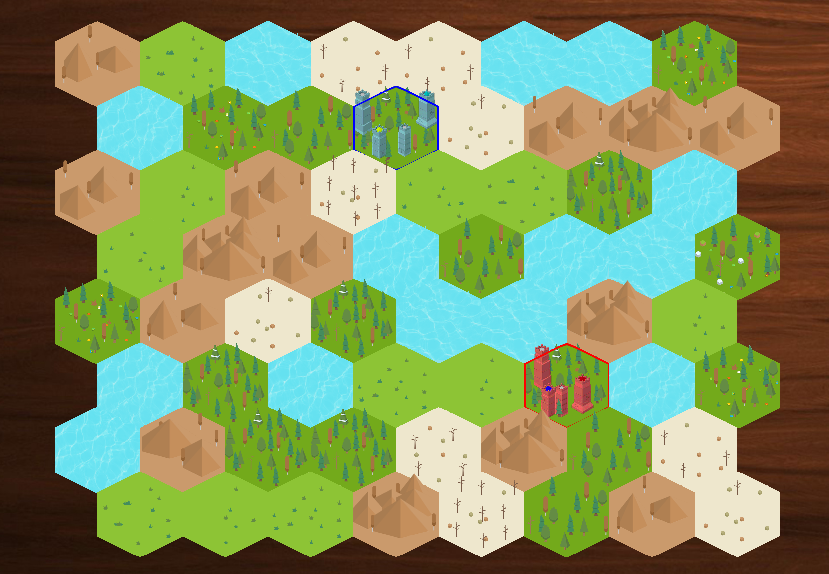
\includegraphics[scale=0.7]{map/random.PNG}

      
      \subsubsection{Map procédurale}
	La map procédurale va générer les différents types de territoires sous forme de biomes. C'est à dire que les territoires ne seront plus placés sans ordre précis, mais les
	territoires de mêmes types vont avoir tendance à se rassembler. Le placement des biomes est lui aléatoire. \\
	Elle prend quatre paramètres :
	\begin{itemize}
	  \item Le nombre de ligne de la map
	  \item Le nombre de colonne de la map
	  \item La taille minimum d'un biome
	  \item La taille maximum d'un biome
	\end{itemize}
	\vspace{0.5cm}
	
	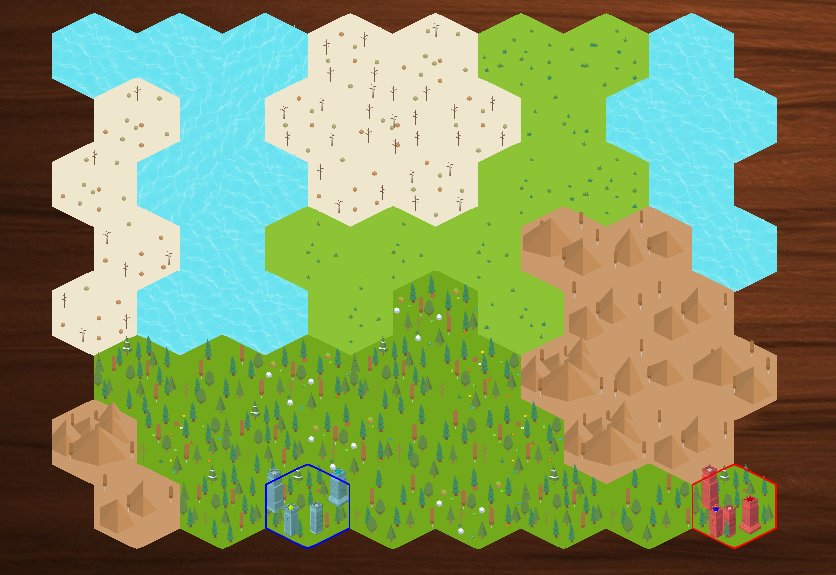
\includegraphics[scale=0.7]{map/procedural.PNG}
	
      \subsubsection{Map générée par le joueur}
	Voir la partie éditeur de la section "graphique"
    
    \subsection{Les phases de jeux}
      Le système de jeu se divisent en plusieurs tours. Chaque tour est divisé en deux phases
      
      \subsubsection{La phase de gestion}
	C'est la phase ou les joueurs vont pouvoir faire leurs différentes actions. Il y a une phase de gestion par joueur par tour.
	
      \subsubsection{La phase de combat}
	Elle commence quand toutes les phases de gestions sont terminées. \\
	On va regarder touts les territoires en conflits, c'est à dire ou des unités d'alliances différentes sont présentes. \\
	On fait le rapport des forces et on détermine le vainqueur (celui qui a le plus de troupes). En cas de forces égalitaires, le vainqueur est tiré au hasard.
    
    \subsection{Les joueurs}
      On peut séparé deux types de joueurs, les joueurs humains et les IA. Ils seront traités de la même façon dans le jeu, seul la manière dont ils font leurs actions changent.
      
      \subsubsection{Les joueurs humains}
	Ils font leurs actions à partir de l'interface graphique pendant les phases de gestion.
    
      \subsubsection{Les IA}
	Leurs actions est calculés par le moteur pendant leurs phases de gestions. On peut définir deux IA de niveaux différentes :
	\begin{itemize}
	 \item \underline{L'IA défensive} : \\
	  C'est une IA basique. Elle va juste chercher à établir des défenses autour de sa position pour empecher l'ennemi de l'atteindre et s'expendre ainsi.
	 \item \underline{L'IA agressive} : \\
	  Cette IA a un comportement qui s'adapte en fonction des actions de(s) adversaire(s). Pour cela nous avons définis des états dans lequel l'IA peut se trouver.
	  Chaque état mène vers un ou plusieurs états en un nombre de tour défini jusqu'à arriver à l'état final recherché (la destruction de la capitale ennemi). \\
	  L'IA va donc appliquer l'algorithme de dijkstra qui est un algorithme très utilisé en pathfinding. Elle va donc pouvoir décider seule des meilleurs actions à faire.
	\end{itemize}

      
      \subsubsection{Les actions possibles}
	Les joueurs peuvent faire plusieurs actions par tour de jeux. En cas d'action impossible, on renvoie une erreur correspondant à l'action. \\
	Les actions possibles sont :
	\begin{itemize}
	 \item Créer/Détruire/Accepter/Rejetter une alliance.
	 \item Créer un batiment sur un territoire vide.
	 \item Créer une troupe dans un batiment militaire
	 \item Déplacer une troupe
	 \item Finir son tour
	\end{itemize}

  
    \subsection{La boucle de jeu}
      La boucle de jeu s'éxécute de la même façon à chaque tour. Elle va mettre en relation tout les éléments ci-dessus :
      \begin{itemize}
       \item On commence par parcourir la map pour produire les ressources de chaques territoires et les donner à leurs possesseurs, pour faire avancer les unités/batiments en constructions etc...
       \item Ensuite on lance la phase de gestion de tout les joueurs et on attend que chaque joueur ai fini son tour
       \item Quand tout le monde a fini son tour, on lance la phase de combat.
       \item Enfin, on regarde si c'est la fin du jeu. Si ce n'est pas le cas on reboucle, sinon on stop et on annonce le vainqueur.
      \end{itemize}
      
    \subsection{Fin du jeu}
      La fin du jeu est déterminée quand il ne reste plus qu'un seul joueur en jeu (Quand il possède donc toutes les capitales). Ce joueur est déclaré vainqueur.
  
  \section{L'interface graphique}
  
  Le graphique est un des pôles les plus important dans la réalisation d'un jeu vidéo, dans notre jeux conquêtes, il a fallut dessiner de nombreux éléments graphiques ainsi que de nombreuses classes graphiques.
  \\
  \\
  \subsection{Les éléments graphiques}
  Au niveau des éléments graphiques, nous pouvons lister :
  \\
  \begin{itemize}
    \item Boutons
    \item Police d'écritures
    \item Images de fond
    \item Textures des territoires
    \item Menu
    \item Skin des soldats
    \item Skins des batiments
    \item Fenêtre de dialogue\\
  \end{itemize}
  
  La police d'écriture du jeu, est la fameuse Korinna, en libre droit d'utilisation, elle fut désigné en 1974, celle-ci est encore utilisé par Disney, Capcom ainsi que de nombreux journaux.
  Une partie des éléments graphiques (arbres, boutons, etc) ont été réalisé par Kenney, un game designer hollandais qui publient des pack de sprites pour des développeurs de jeux vidéos, il va de soi que les packs que nous avons utilisés sont libre de droits.
  Pour la réalisation et l'assemblage des éléments graphique, nous avons utilisé exclusivement GIMP sous Windows, ce qui nous à permis d'adapter les divers éléments graphiques à nos besoin.
  
  \subsection{Les classes graphiques}
Au niveau des classes générant un rendu graphique, nous les avons mis dans un dossier screen, et elles commencent toutes par Gui.
\\
\\
  Voici la listes avec leur descriptions respectives :
  \\
  \begin{itemize}
    \item GuiEditor
      GuiEditor nous permet d'accéder au mode éditeur. Le mode éditeur nous permet de créer notre propre map avec les types de territoires, capitales etc.\\
    \item GuiGame
      GuiGame est la classe la plus importante de notre projet, en effet, celle-ci gère l'affichage complet du jeux.\\
    \item GuiHelp
      GuiHelp est une page d'aide pour l'utilisateur accessible via le bouton aide dans GuiGame.\\
    \item GuiLoading
      GuiLoading nous affiche la page de chargement de parties.
    \item GuiMenu
      GuiMenu gère l'affichage et les interactions de l'utilisateur avec le menu principal du jeu.\\
    \item GuiResult
      GuiResult s'affiche en fin de partie, celle-ci annonce la fin de la partie et propose au joueur de rejouer.\\
    \item GuiSettings
      GuiSettings comme son nom l'indique permet d'accéder aux menu de réglages du jeux.\\
    \item GuiStream
     GuiStream est l'interface qui permettant de rediriger les messages d'erreurs vers la  fenêtre graphique.\\
  \end{itemize}
  
  \subsection{Les extensions}
    Nous avons dans notre projet réussi à réaliser deux extensions du cahier des charges :
    \subsubsection{Mise en place des langues}
      Nous avons mise en place un système de fichier de localisations. Il nous est donc possible de changer de langue n'importe quand pendant le jeu. Pour l'instant les langues gérées sont
      l'anglais et le français mais il nous est très simple d'en rajouter.
      
    \subsubsection{Mise en place du réseau}
      Nous avons aussi mis en place une surcouche réseau "Serveur/Client" dans notre jeu. Le serveur communique avec le moteur et le client avec l'interface graphique.
      Il est donc possible de jouer jusqu'à 8 joueurs en même temps sur 8 postes différents. Cela accèlère la vitesse des parties
  
  \chapter{Manuel Utilisateur}
    Age of Swag : Conquest CMI est un jeu amateur libre et gratuit conçu par des étudiants à l'Université de Cergy-Pontoise, développé en Java à l'aide de la librairie graphique LibGdx.\\

Avant de vous lancer dans l'aventure de Age of Swag, nous vous recommandons de lire ce mode d'emploie pour savoir comment jouer mais aussi connaître les conseils indispensables.\\

Age of Swag vous propose un support technique gratuit et hors pair, disponible 24/24h 7/7j aux adresses mails suivantes :\\
  \begin{itemize}
    \item bastien-12@hotmail.fr
    \item lucas.nicosia@yahoo.fr
    \item aryus96@hotmail.fr
  \end{itemize}
    
    Attention, cette assistance s'adresse seulement aux bénéficiaires de notre projet Age Of Swag.\\

\section{Configuration requise}
Age of Swag : Conquest CMI fonctionne sur divers systèmes
tels que Windows, Linux ou Mac OS X. Etant libre, elle peut être facilement
portée sur d'autres systèmes (contactez-nous).
Nous avons fait de notre mieux pour optimiser la programmation, mais le
jeu utilise tout de même un minimum de ressources, donc il risque de ne
pas être jouable correctement sur des ordinateurs relativement peu
puisssants.
Les performances diffèrent selon les machines et il est difficile d'établir
précisément une configuration minimale. Nous vous conseillons quoi qu'il
en soit de fermer toutes les autres applications actives quand vous jouez à
Age Of Swag : Conquest CMI.\\

Age Of Swag à été testé sur divers configuration, et à été jugé parfaitement fonctionnel par notre équipe sur ces configurations :\\
  \begin{itemize}
    \item i7-3630QM (2.4Ghz)- Nvidia GT740M - 16Go de RAM
    \item i5-3230M (2.6GHz) - Nvidia NVS 5200M - 8Go de RAM
    \item i5 650 (3.20Ghz )- AMD Radeon HD 5700 Series - 4Go de RAM\\
  \end{itemize}
  \section{Configuration le jeu}
  \textbf{Installer Age of Swag : Conquest CMI}\\
  
  Pour installer et démarrer Age Of Swag, rien de plus simple, il suffit d'installer la dernière Java Runtime Environment (Pour plus d'informations sur l'obtention de la derniere Java Runtime Environment, connectez-vous à l'adresse suivante \url{http://www.oracle.com/technetwork/java/javase/downloads/jre8-downloads-2133155.html}.

  Si vous disposez déjà de Java Runtime Environment ou que vous venez de l'installer, il vous suffit juste de double cliquer sur l'exécutable .jar du projet.\\
  
    \textbf{Désinstaller Age of Swag : Conquest CMI}\\
    
    Il vous suffit de supprimer l'exécutable .jar .\\
    
    \section{Jouer à Age of Swag : Conquest CMI}
	     
    \underline{Modes de jeu}\\ 
     
 \begin{enumerate}
\item Normal
 Dans ce mode, la carte est généré aléatoirement mais vous pouvez choisir le nombre de joueurs humain, le nombre de joueurs géré par l'ordinateur et si vous voulez qu'ils soient agressifs ou défensifs.\\
\item Aléatoire.\\
 Dans ce mode, la carte est généré aléatoirement, vous pouvez choisir le nombre de joueurs humain, ainsi que ceux gérés par l'ordinateur mais vous ne pouvez pas choisir leurs stratégies de combats.\\
\end{enumerate}     
     
     \underline{Local}\\
     
     \begin{enumerate}
\item Démarrez le jeu.
\item Appuyez sur le 1er bouton, New Game/Nouvelle partie.
\item Appuyez sur Local.
\item Dès lors, choisissez votre mode de jeux.\\
\end{enumerate}
     
     \underline{En ligne}\\
         \begin{enumerate}
\item Démarrez le jeu.
\item Appuyez sur le 1er bouton, New Game/Nouvelle partie.
\item Appuyez sur Online.
\item Choisissez si vous créez la partie ou rejoignez une partie.\\
\end{enumerate}
    
     \underline{Charger une partie}\\
         \begin{enumerate}
\item Démarrez le jeu.
\item Appuyez sur le 2nd bouton,Load game/Charger une partie.
\item Sélectionnez votre partie précédemment enregistré.
\end{enumerate}


     \underline{Editeur}\\
         \begin{enumerate}
\item Démarrez le jeu.
\item Appuyez sur le 3ème bouton,Load game/Charger une partie.
\item Créer votre carte avec le nombre de joueurs voulu.\\
\end{enumerate}


\section{Autres informations}

 \underline{Remporter la partie}\\
Pour gagner la partie, vous devrez conquérir l'intégralité des capitales ennemis à l'aide de vos troupes.\\
 
 \underline{Former une unité}\\
Afin de former une unité vous devez sélectionner votre capitale ou bien un territoire possédant une caserne. Vérifiez que vous avez bien les ressources nécessaire à sa formation, puis patienter le nombre de tours exigé pour l'unité. Attention, les casernes et capitales ne peuvent former que une unité à la fois.\\
  
   \underline{Créer un bâtiment}\\
Afin de créer un bâtiment, vous devez sélectionner un territoire autre que votre capital, vous appartenant et appuyer sur le bouton de création du bâtiment souhaité, attention, vérifier bien d'avoir les ressources nécessaires, puis vous devrez patienté un certains nombre de tour. \\
 
 \underline{Taille de la carte}
 La taille de la carte dans le mode éditeur est fixe.
 La taille dans les autres modes dépends du nombre de joueurs que vous mettez dans la partie.\\
 \\
 \underline{Types de territoires}\\
 \\
 Il existe 5 types de territoires : \\
 \begin{itemize}
    \item Forestier\\
    
\includegraphics[scale=0.31]{ground/fo.png}\\
    \item Montagneux\\
    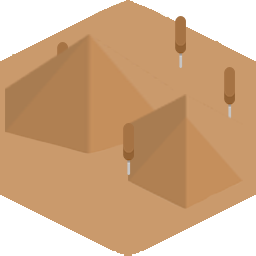
\includegraphics[scale=0.31]{ground/mo.png}\\
    \item Désertique\\
    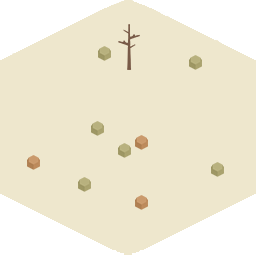
\includegraphics[scale=0.31]{ground/de.png}\\
    \item Aquatique\\
    
\includegraphics[scale=0.31]{ground/wa.png}\\
    \item Plaine\\
    
\includegraphics[scale=0.31]{ground/pl.png}\\
  \end{itemize}
    Les territoires Désertique et aquatiques sont les seuls qui vous seront infranchissable.\\
  \\
  \underline{Types de troupes}\\
  Age of Swag dispose actuellement de 5 types de troupes :\\
   \begin{itemize}
    \item    
\includegraphics[scale=0.31]{troops/bow.png} Archer\\
   L'archer sera intéressant par son faible coût, temps de production et son attaque.\\
    ATK : 15\\
    DEF : 10\\
    2 tours de constructions et un coût de 20 ressources.\\
    
    \item 
\includegraphics[scale=0.31]{troops/wiz.png} Magicien\\
     Le magicien possède la plus grande puissance d'attaque mais son coût et temps de production font de lui une arme stratégique.\\
    ATK : 25\\
    DEF : 5\\
    3 tours de constructions et un coût de 30 ressources.\\
    
    \item 
\includegraphics[scale=0.31]{troops/sword.png}  Épéiste\\
         L'épéiste tient sa force dans sa neutralité, l'équilibre de ces caractéristiques font de lui un soldat de choix.\\
    ATK : 15\\
    DEF : 15\\
    2 tours de constructions et un coût de 25 ressources.\\
    
    \item 
\includegraphics[scale=0.31]{troops/spear.png}  Lancier\\
             Le Lancier est une troupe de choix dans le cas d'une défense de territoire.\\
    ATK : 10\\
    DEF : 20\\
    2 tours de constructions et un coût de 25 ressources.\\
    \item 
\includegraphics[scale=0.31]{troops/barbare.png}  Barbare\\
                 Le barbare est le soldat le plus basique du jeux. Il est néanmoins intéressant par sa rapidité de production et son faible coût.\\
    ATK : 10\\
    DEF : 10\\
    1 tours de constructions et un coût de 20 ressources.\\
  \end{itemize}

  \underline{Types de bâtiments}\\
  Age Of Swag : Conquest CMI dispose également de 3 types de bâtiments. \\
     \begin{itemize}
    \item l'Usine\\
    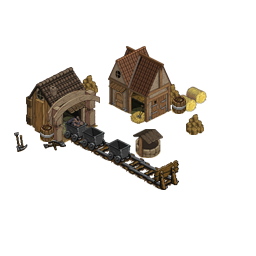
\includegraphics[scale=0.3]{bat/fac.png}\\
  L'usine va permettre d'augmenter la production des ressources sur le territoire sur lesquels vous l'avez construits, attention toutefois, chaque territoires possèdent un stock de ressources, il est judicieux de placer des usines à certains endroits.\\
    
    \item Caserne\\
    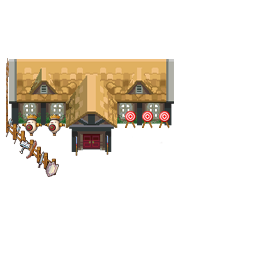
\includegraphics[scale=0.3]{bat/bar.png}\\
     La caserne vous permettras de créer des troupes hors de la capitale mais aussi de produire d'avantage de troupes par tours.\\
    
    \item Défense\\
    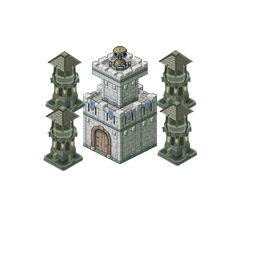
\includegraphics[scale=0.3]{bat/ram.png}\\
         Le bâtiment de défense va permettre à vos troupes de gagner en défense et donc de mieux résister aux assauts des troupes ennemis.\\
    
  \end{itemize}
   \textbf{Interface }\\
 \\
  \begin{center}
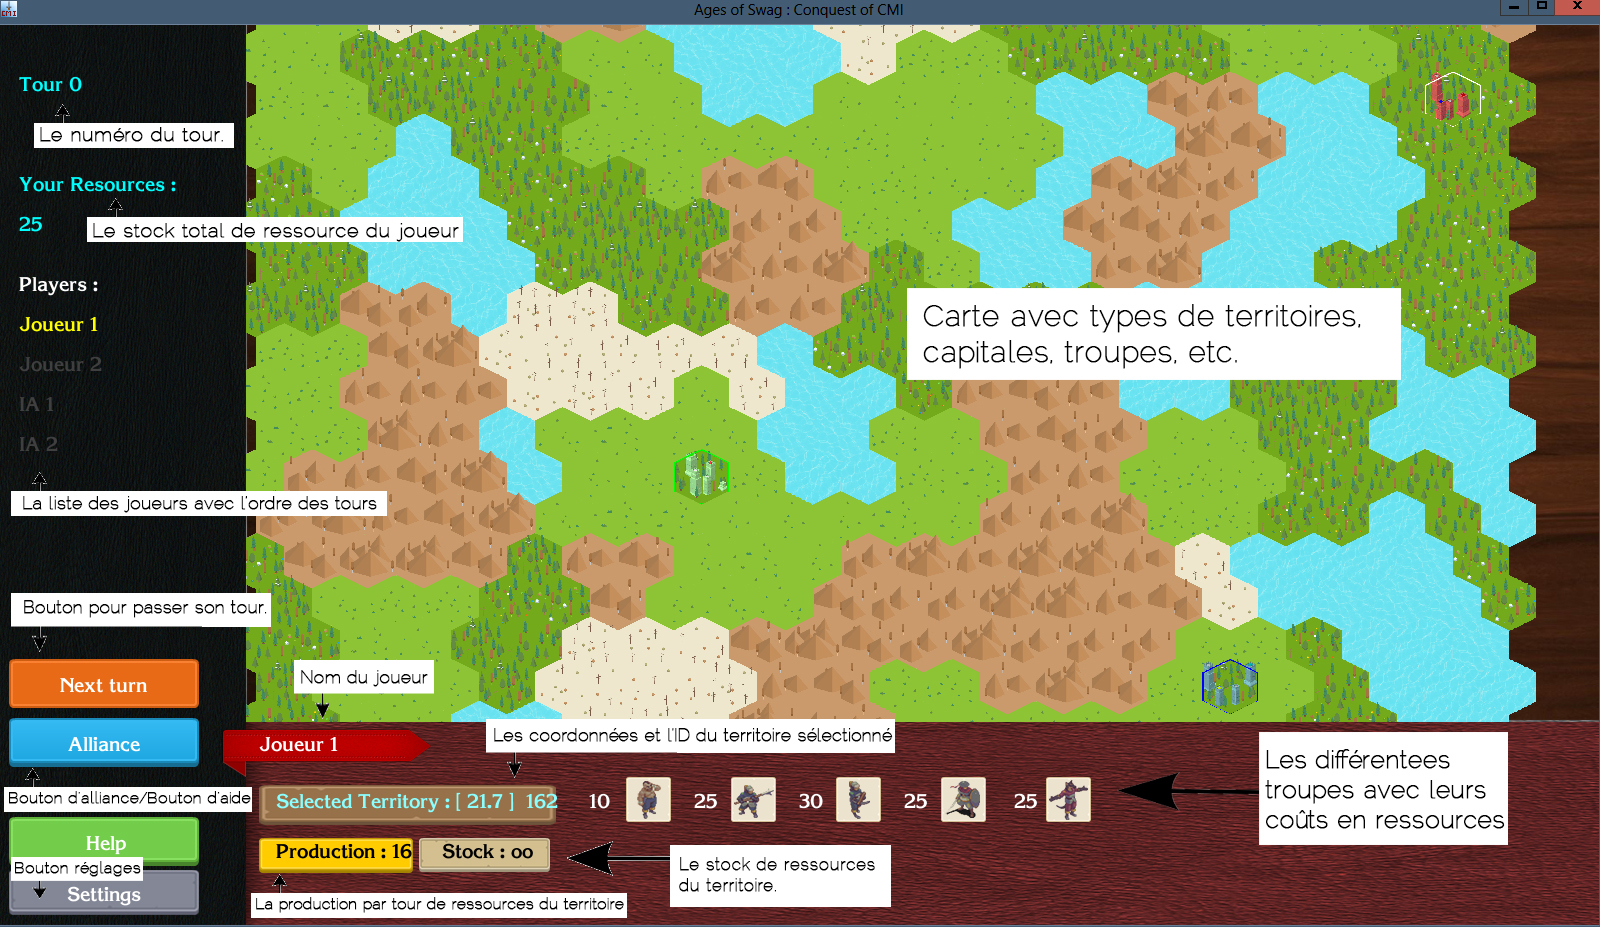
\includegraphics[scale=0.31]{help.jpg} \\
\end{center}

   \textbf{Modifier les options de jeu}\\

Les options de Age Of Swag sont relativement basique, vous avez la possibilité de changer la langue du jeu mais aussi de désactiver le son (seulement à partir du menu principal).\\
   
   \textbf{Pour afficher l'aide}\\
   Si vous souhaitez avoir de l'aide et des informations lors du jeux, vous pouvez cliquer sur le bouton vert aide/help qui vous donneras un panel d'informations sur le fonctionnement du jeu.

  \chapter{Déroulement du projet}
    \section{La conception}
La conception fut l'étape clé pour notre projet de Génie Logiciel, en effet, impossible de se lancer dans un projet d'une telle envergure sans une étape de conception.
Il a fallu tout d'abord concevoir les données que nous allions utiliser, pour cela, nous avons réaliser un diagramme de classe avec l'intégralité des données utilisable et qui vont être traitées par notre programme.
Nous avons également réfléchis à l'interface graphique et le style de jeu que nous souhaitions afin de ne pas devoir changer plus tard dans le projet.
Nous avons également réfléchis aux méthodes et aux techniques de traitements que nous allions utiliser pour nos données, celles qui serait le plus rapide, d'une part pour nous à réaliser mais aussi pour les performances de l'ordinateur.


\section{La concrétisation}

Une fois l'étape de conception finalisée, il nous fut facile de le concrétiser car le projet comporte de nombreuses parties que nous nous sommes partagé afin d'avoir un travail et une organisation efficiente.
Nous avons évidemment commencer par réaliser l'intégralité des données.
Par la suite, nous avons commencé à les traiter, dès lors que cela prenais de la forme,il fut crucial d'entamer la création d'une interface graphique afin de pouvoir avoir un meilleur rendu et affichage de notre travail.
Par la suite, plus notre projet prenais forme, plus la nécessité d'avoir un menu fut important



\section{Finalisations et améliorations}

Les finalisations d'un jeu vidéos sont innombrables,il n'y à qu'a voir les jeux d'aujourd'hui, même après leur sortie, ils requièrent des mise à jours régulières. Pour notre part, les plus grosses finalisations furent pour l'interactivité du jeu, la facilité pour l'utilisateur de comprendre et de pouvoir jouer au jeu, car de notre point de vu développeur, le jeu parait très facile à jouer car nous l'avons développé. Nous avons donc demandé à des cobayes d'essayer de jouer à Age Of Swag, et nous avons vite remarqué que le jeu était en réalité plus compliqué à comprendre pour un nouveau joueur, il nous à donc fallut rajouter une page d'aide, d'avantage de boutons, etc.

Le projet conquête est débordant d'imagination, en effet, de part son côté jeu vidéo et de notre expérience dans ce domaine, nos idées d'améliorations furent nombreuses. Toutefois par des soucis de temps et non pas de compétences, nous avons préféré nous concerter sur les plus importantes que je vais vous présenter.
Nous avons implémenté le jeux en réseau, vous pouvez dès lors jouer avec plusieurs ordinateurs sur la même partie.
Nous avons également rajouter une musique lorsque vous lancez Age Of Swag, en effet, l'absence de musique rendait le jeu moins attrayant. Afin de rendre le gameplay du jeu plus attrayant et agréable, nous avons implémenté différents types de troupes et inclut la possibilité pour le joueur de créer des bâtiments.
L'interface graphique à été également peaufiné tout au long du projet afin d'être le plus attractif et intuitif pour l'utilisateur, au delà d'une interface graphique simple, il y a toute une recherche et réflexion derrière la réalisation de l'interface, des choix des couleurs, images, etc.

  
  \chapter{Conclusion}
    Pour conclure, à travers le génie logiciel et notre projet conquête, nous avons gagné en professionnalisation en effet, nous avons appris à :\\

  \begin{itemize}
    \item Réaliser un projet complexe en groupe
    \begin{itemize}
    	\item Pas loin de 8000 lignes de code.
    	\item 144 classes.
    	\item 230 images.
    	\item Des centaines d'heures de travail.\\
    	\end{itemize}
    \item approfondir les techniques de conception et de programmation\\
    \item maitriser les différents outils de réalisation de logiciels : 
    	\begin{itemize}
    	\item utilisation avancée d'Eclipse
    	\item SVN
    	\item Junit
    	\item Log4j\\
    	\end{itemize}
  \end{itemize}
Au delà  de l'aspect éducatif que nous à apporté le génie logiciel, cela nous a permis de former un groupe de travail productif dans lesquels chacun de nous à pris plaisir à travailler et à s'épanouir au fur et à mesure du projet.
    
    \chapter{Remerciements}
<<<<<<< .mine
Nous tenons à remercier notre enseignant tuteur, Monsieur Tianxiao LIU qui nous a été d'une aide précieuse et qui nous a consacré du temps. De plus, nous tenons à remercie Madame Tuyêt Trâm DANG NGOC, qui a lancé le module de Génie Logiciel.=======
Nous tenons à remercier :
\begin{itemize}
 \item Notre enseignant tuteur, Monsieur Tianxiao LIU qui nous a été d'une aide précieuse et qui nous a consacré du temps.
 \item Madame Tuyêt Trâm DANG NGOC, qui a lancé le module de Génie Logiciel.
 \item La promotion L2 CMI SIC et plus généralement tout le groupe A pour cette chaleureuse ambiance et cet esprit d'entraide.
\end{itemize}>>>>>>> .r146


\end{document}
